\subsection{Block HQR with partitioned rows : Tall-and-Skinny QR (TSQR)}\label{sec:TSQR}
Some important problems that require QR factorizations of overdetermined systems include least squares problems, eigenvalue problems, low rank approximations, as well as other matrix decompositions.
Although Tall-and-Skinny QR (TSQR) broadly refers to block QR factorization methods with row partitions, we will discuss a specific variant of TSQR which is also known as the AllReduce algorithm \cite{Mori2012}.
In this paper, the TSQR/AllReduce algorithm refers to the most parallel variant of the block QR factorization algorithms discussed in \cite{Demmel2012}.
A detailed description and rounding error analysis of this algorithm can be found in \cite{Mori2012}, and we present a pseudocode for the algorithm in \cref{algo:par_tsqr}.
Our initial interest in this algorithm came from its parallelizable nature, which is particularly suitable to implementation on GPUs. 
Additionally, our numerical simulations (discussed in \cref{sec:NE}) show that TSQR can not only increase the speed but also outperform the traditional HQR factorization in low precisions.
\subsubsection{TSQR/AllReduce Algorithm}
\Cref{algo:par_tsqr} partitions the rows of a tall-and-skinny matrix, $\bb{A}$. 
HQR is performed on each of those blocks and pairs of $\bb{R}$ factors are combined to form the next set of $\bb{A}$ matrices to be QR factorized. 
This process is repeated until only a single $\bb{R}$ factor remains, and the $\bb{Q}$ factor is built from all of the HH constants and vectors stored at each level.
The most gains from parallelization can be made in the initial level where the maximum number of independent HQR factorizations occur. 
Although more than one configuration of this algorithm may be available for a given tall-and-skinny matrix, the number of nodes available and the shape of the matrix eliminate some of those choices. 
For example, a 1600-by-100 matrix can be partitioned into 2, 4, 8, or 16 initial row-blocks but may be restricted by a machine with only 4 nodes, and a 1600-by-700 matrix can only be partitioned into 2 initial blocks.
Our numerical experiments show that the choice in the initial partition, which directly relates to the recursion depth of TSQR, has an impact in the accuracy of the QR factorization. \par

We refer to \emph{level} as the number of recursions in a particular TSQR implementation. 
An $L$-level TSQR algorithm partitions the original matrix into $2^{(l)}$ submatrices in the initial or $0^{th}$ level of the algorithm, and $2^{L-i}$ QR factorizations are performed in level $i$ for $i = 1 , \cdots, L$. 
The set of matrices that are QR factorized at each level $i$ are called $\bb{A}_j^{(i)}$ for $j = 1, \cdots, 2^{L-i}$, where superscript $(i)$ corresponds to the level and the subscript $j$ indexes the row-blocks within level $i$.
In the following sections, \cref{algo:par_tsqr} ({\tt tsqr}) will find a TSQR factorization of a matrix $A\in\R^{m\times n}$ where $m \gg n$. 
The inline function {\tt qr} refers to \cref{algo:hhQR} and we use \cref{algo:hh_v2} as a subroutine of {\tt qr}.

\paragraph{TSQR Notation}
We introduce new notation due to the multi-level nature of the TSQR algorithm.
In the final task of constructing $\bb{Q}$, $\bb{Q}_j^{(i)}$ factors are aggregated from each block at each level.
Each $\bb{Q}_j^{(i)}$ factor from level $i$ is partitioned such that two corresponding $\bb{Q}^{(i-1)}$ factors from level $i-1$ can be applied to them. 
The partition (approximately) splits $\bb{Q}_{j}^{(i)}$ into two halves, $[\tilde{\bb{Q}}_{j, 1}^{(i)\top} \tilde{\bb{Q}}_{j, 2}^{(i)\top}]^{\top}$.
The functions $\alpha(j)$ and $\phi(j)$ are defined such that $\bb{Q}_j^{(i)}$ is applied to the correct blocks from the level below: $\tilde{\bb{Q}}_{\alpha(j), \phi(j)}^{(i+1)}$.
For $j = 1 , \cdots, 2^{L-i}$ at level $i$, we need $j = 2(\alpha(j)-1) + \phi(j)$, where $\alpha(j) = \lceil \frac{j}{2}\rceil$ and $\phi(j) = 2 + j - 2\alpha(j) \in\{1,2\}$.
\cref{Qdetails} shows full linear algebra details for a single-level ($L=1$, $2$ initial blocks) example.
The reconstruction of $\bb{Q}$ can be implemented more efficiently (see \cite{BDGJNS2014}), but the reconstruction method in \cref{algo:par_tsqr} is presented for a clear, straightforward explanation.

\begin{algorithm2e}[H]
	\DontPrintSemicolon 
	\KwIn{$\bb{A}\in\R^{m \times n}$ where $m \gg n$, $L\leq\lfloor\log_2\left(\frac{m}{n}\right)\rfloor$, and $2^L$ is the initial number of blocks. }
	
	\KwOut{$\bb{Q}\in\R^{m \times n}$, $\bb{R} \in\R^{n\times n}$ such that 	$\bb{Q}\bb{R} = \bb{A}$.}
	$h \gets \lfloor \frac{m}{2^L} \rfloor$ \tcp*{Number of rows.}
	%$r \gets m - (2^L-1)h$ \tcp*{Number of rows for the last block ($h\leq r <2h$).}
	\tcc{Split $\bb{A}$ into $2^L$ blocks. Note that level $(i)$ has $ 2^{L-i}$ blocks.}
	\For {$j = 1 : 2^L$}{
		$\bb{A}_j^{(0)} \gets \bb{A}[(j-1)h+1: jh, :]$ 
	}
	%$\bb{A}_{2^L}^{(0)} \gets \bb{A}[(2^L-1)h:m, :]$ \tcp*{Last block may have more rows.} 
	\tcc{Store Householder vectors as columns of matrix $\bb{V}_j^{(i)}$, Householder constants as components of vector $\bm{\beta}_j^{(i)}$, and set up the next level.}
	\For{$i = 0 : L-1$}{
		\tcc{The inner loop can be parallelized.}
		\For {$j = 1 : 2^{L-i}$ }{
			$\bb{V}_{2j-1}^{(i)}$, $\bm{\beta}_{2j-1}^{(i)}$, $\bb{R}_{2j-1}^{(i)} \gets{\tt qr}(\bb{A}_{2j-1}^{(i)})$ \;
			$\bb{V}_{2j}^{(i)}$, $\bm{\beta}_{2j}^{(i)}$, $\bb{R}_{2j}^{(i)} \gets{\tt qr}(\bb{A}_{2j}^{(i)})$
			\(\bb{A}_{j}^{(i+1)} \gets \begin{bmatrix}
			\bb{R}_{2j-1}^{(i)}\\
			\bb{R}_{2j}^{(i)}
			\end{bmatrix}\)
		}
	}
	$\bb{V}_{1}^{(L)}$, $\bm{\beta}_1^{(L)}$, $\bb{R}  \gets{\tt qr}(\bb{A}_{1}^{(L)})$ \tcp*{The final $\bb{R}$ factor is built.}
	$\bb{Q}_{1}^{(L)} \gets {\tt hh\_mult}(\bb{V}_{1}^{(L)}, I_{2n\times n})$\;
	\tcc{Compute $\bb{Q}^{(i)}$ factors by applying $\bb{V}^{(i)}$ to $\bb{Q}^{(i+1)}$ factors.}
	\For {$i = L-1 : -1 : 1$}{
		\For {$j = 1 : 2^{L-i}$}{
			\(\bb{Q}_{j}^{(i)} \gets {\tt hh\_mult}\left(\bb{V}_{j}^{(i)}, \begin{bmatrix}
			\tilde{\bb{Q}}_{\alpha(j), \phi(j)}^{(i+1)}\\
			\bb{0}_{n,n}
			\end{bmatrix}\right)\)
		}
	}
	%\tcc{At the top-most level, construct the final $\bb{Q}$ factor.}% from $\bb{Q}^{0}$ factors.}
	$\bb{Q} \gets [];$\tcp*{Construct the final $\bb{Q}$ factor.}
	\For{$ j = 1 : 2^L $}{
		\(\bb{Q} \gets \begin{bmatrix}
		\bb{Q} \\
		{\tt hh\_mult}\left(\bb{V}_{j}^{(0)} , \begin{bmatrix}
		\tilde{\bb{Q}}_{\alpha(j), \phi(j)}^{(1)}\\
		O_{\tilde{h},n}
		\end{bmatrix} \right)
		
		\end{bmatrix}\)
		}
	\Return{$\bb{Q}$, $\bb{R}$}
	\caption{$\bb{Q},\bb{R}={\tt tsqr}(\bb{A}, L)$.  Finds a QR factorization of a tall, skinny matrix, $\bb{A}$. }
	\label{algo:par_tsqr}
\end{algorithm2e}
\subsubsection{Single-level Example}
\label{Qdetails}
In the single-level version of this algorithm, we first bisect $\bb{A}$  into $\bb{A}_1^{(0)}$ and $\bb{A}_2^{(0)}$ and compute the QR factorization of each of those submatrices.
We combine the resulting upper-triangular matrices (see below)
% , i.e.,  \(\bb{A}_{1}^{(1)} =\begin{bmatrix}
%\bb{R}_{1}^{(0)}\\ 
%\bb{R}_{2}^{(0)} 
%\end{bmatrix},\)   
which is QR factorized, and the process is repeated:
\[
\bb{A} = \begin{bmatrix}
\bb{A}_1^{(0)}\\
\bb{A}_2^{(0)}
\end{bmatrix} = \begin{bmatrix}
\bb{Q}_1^{(0)}\bb{R}_1^{(0)}\\
\bb{Q}_2^{(0)}\bb{R}_2^{(0)}
\end{bmatrix} = \begin{bmatrix}
\bb{Q}_1^{(0)} & \bb{0}\\
\bb{0} & \bb{Q}_2^{(0)}
\end{bmatrix} \begin{bmatrix}
\bb{R}_1^{(0)} \\
\bb{R}_2^{(0)}
\end{bmatrix} =\begin{bmatrix}
\bb{Q}_1^{(0)} & \bb{0}\\
\bb{0} & \bb{Q}_2^{(0)}
\end{bmatrix} \bb{A}_1^{(1)} =\begin{bmatrix}
\bb{Q}_1^{(0)} & \bb{0}\\
\bb{0} & \bb{Q}_2^{(0)}
\end{bmatrix} \bb{Q}_1^{(1)}\bb{R}.
\] 
The $\bb{R}$ factor of $\bb{A}_1^{(1)}$ is the final $\bb{R}$ factor of the QR factorization of the original matrix, $\bb{A}$. 
However, the final $\bb{Q}$ still needs to be constructed.
Bisecting  $\bb{Q}_1^{(1)}$ into two submatrices, i.e. $\tilde{\bb{Q}}_{1,1}^{(1)}$ and $\tilde{\bb{Q}}_{1,2}^{(1)}$, allows us to write and compute the product more compactly,  \[
\bb{Q}:=\begin{bmatrix}
\bb{Q}_1^{(0)} & \bb{0}\\
\bb{0} & \bb{Q}_2^{(0)}
\end{bmatrix} \bb{Q}_1^{(1)} =    \begin{bmatrix}
\bb{Q}_1^{(0)} & \bb{0}\\
\bb{0} & \bb{Q}_2^{(0)}
\end{bmatrix} \begin{bmatrix}
\tilde{\bb{Q}}_{1,1}^{(1)}\\
\tilde{\bb{Q}}_{1,2}^{(1)}
\end{bmatrix}= \begin{bmatrix}
\bb{Q}_1^{(0)}\tilde{\bb{Q}}_{1,1}^{(1)} \\ 
\bb{Q}_2^{(0)}\tilde{\bb{Q}}_{1,2}^{(1)}
\end{bmatrix}. \]
More generally, \cref{algo:par_tsqr} takes a tall-and-skinny matrix $\bb{A}$ and level $L$ and finds a QR factorization by initially partitioning $\bb{A}$ into $2^{(l)}$ row-blocks and includes the building of $\bb{Q}$.
For simplicity, we assume that $m$ is exactly $h2^{(l)}$ so that the initial partition yields $2^{(l)}$ blocks of equal sizes, $h$-by-$n$. 
Also, note that {\tt hh\_mult} refers to the action of applying multiple HH transformations given a set of HH vectors and constants, which can be performed by iterating line 6 of \cref{algo:hhQR}.
This step can be done in a level-3 BLAS operation via a WY update if \cref{algo:par_tsqr} was modified to store the WY representation at the QR factorization of each block of each level, $\bb{A}_j^{(i)}$. 

\subsubsection{TSQR: Rounding Error Analysis}
\label{sec:TSQRre}
The TSQR algorithm presented in \cref{algo:par_tsqr} is a divide-and-conquer strategy for the QR factorization that uses the HQR within the subproblems. 
Divide-and-conquer methods can naturally be implemented in parallel and accumulate less rounding errors.
For example, the single-level TSQR decomposition of a tall-and-skinny matrix, $\bb{A}$ requires 3 total HQRs of matrices of sizes $\lfloor\log_{2}(\frac{m}{n})\rfloor$-by-$n$, $\lceil\log_{2}(\frac{m}{n})\rceil$-by-$n$, and $2n$-by-$n$.
The single-level TSQR strictly uses more FLOPs, but the dot product subroutines may accumulate smaller rounding errors (and certainly have smaller upper bounds) since they are performed on shorter vectors, and lead to a more accurate solution overall.
These concepts are elucidated in \cite{Mori2012} and we summarize the main results  in \cref{thm:moriTSQR}.

\begin{theorem}
	\label{thm:moriTSQR}
	Let $\bb{A}\in\R^{m\times n}$ with $m\geq n$ have full rank, $n$, and $\hat{\bb{Q}}_{TSQR}\in\R^{m\times n}$ and $\hat{\bb{R}}_{TSQR}\in\R^{n\times n}$ be the thin QR factors of $\bb{A}$ obtained via \cref{algo:par_tsqr} with $L$ levels. 
	Let us further assume that $m$ is divisible by $2^L$ and $n\tilde{\gamma}_{m2^{-L}}, n\tilde{\gamma}_{ 2n} \ll 1$.
	Then, 2-norm error bound for the $j^{th}$ column ($j=1:n$) of $\hat{\bb{R}}_{TSQR}$ and the Frobenius norm error bound for $\hat{\bb{Q}}_{TSQR}$ are
	\begin{align}
	\|\hat{\bb{R}}_{TSQR}[:,j]-\bb{R}[:,j]\|_2 &\leq n(\tilde{\gamma}_{m2^{-L}} + L\tilde{\gamma}_{ 2n})\|\bb{A}[:,j]\|_2,  \label{eqn:tsqrRA}\\
	\|\hat{\bb{Q}}_{TSQR}-\bb{Q}\|_F &\leq n^{3/2}(\tilde{\gamma}_{m2^{-L}} + L\tilde{\gamma}_{ 2n}).\label{eqn:tsqrQ}
	%\|\hat{\bb{Q}}_{TSQR}[:,j]-\bb{Q}[:,]\|_2 &\leq n(\tilde{\gamma}_{m2^{-L}} + L\tilde{\gamma}_{ 2n}).\label{eqn:tsqrQ}
	\end{align}
\end{theorem}

Note that the $n\tilde{\gamma}_{m2^{-L}}$ and $n\tilde{\gamma}_{ 2n}$ terms correspond to errors from applying HQR to the blocks in the initial partition and to the blocks in levels 1 through $L$ respectively.
We can easily replace these with analogous mixed precision terms and keep the analysis accurate.
Both level-2 and level-3 BLAS implementations will be considered in \cref{sec:mpanalysis}.
\paragraph{TSQR and HQR error bound comparison}
%\subsubsection{HQR and TSQR error bound comparison}
%\label{sec:HTSQR}
We compare the error bounds for HQR and TSQR. 
%\paragraph{Uniform precision comparison}
Consider the bounds for $\|\hat{\bb{Q}}-\bb{Q}\|_F$ in \cref{thm:feHQR,thm:moriTSQR}.
%In order for the a meaningful TSQR error bound to outperform the bound for the HQR algorithm, 
TSQR has a lower worst-case error bound than HQR when integers $m, n > 0$, and $L\geq0$ satisfy
\begin{equation*}
1\gg n^{3/2}\gamma^{(m)} \gg n^{3/2}(\gamma^{(\frac{m}{2^L})}+L\gamma^{(2n)}).
\end{equation*}
%for TSQR to have a better worst-case error bound than HQR.
Let us consider as an example the case when $\frac{m}{2^L}=2n$.
Then, the HQR bound is $2^L/(L+1)$ larger than the bound for TSQR with $L$ levels. 
%TODO: O
For example, in single precision, a HQR of a $2^{15}$-by-$2^6$ matrix results in an upper bound relative backward error ($\|\bb{A}-\hat{\bb{Q}}\hat{\bb{R}}\|_F/\|\bb{A}\|_F$) of $\approx${\tt1.002}, but a TSQR with $L=8$ is bounded by $\approx${\tt 3.516e-02}. 
This case exemplifies a situation in which stability is not guaranteed in HQR, but the method is stable when using TSQR, even in the worst-case. 
Now consider some $2^{20}$-by-$2^{12}$ matrix and QR factorizations performed with double precision.
The error bound for HQR is {\tt 1.686e-7}, whereas the error bound for TSQR with 12 levels is {\tt 5.351e-10}.
In general, we can conjecture that values of $L$ that can make $m2^{-L}$ and $2Ln$ much smaller than $m$, should produce a TSQR that outperforms HQR in worst-case scenarios, at least in uniform precision settings.
However, the range of matrix sizes that TSQR can accommodate decreases as $L$ grows larger.
%, and the range is only half of that of HQR even for a single-level TSQR. 
Figure~\ref{fig:paramspace} shows the matrix sizes HQR, 2-level TSQR, and 4-level TSQR can accommodate as well as their respective error bounds.\par
\begin{wrapfigure}{l}{.45\textwidth}
	\centering
	%\vspace{-15pt}
	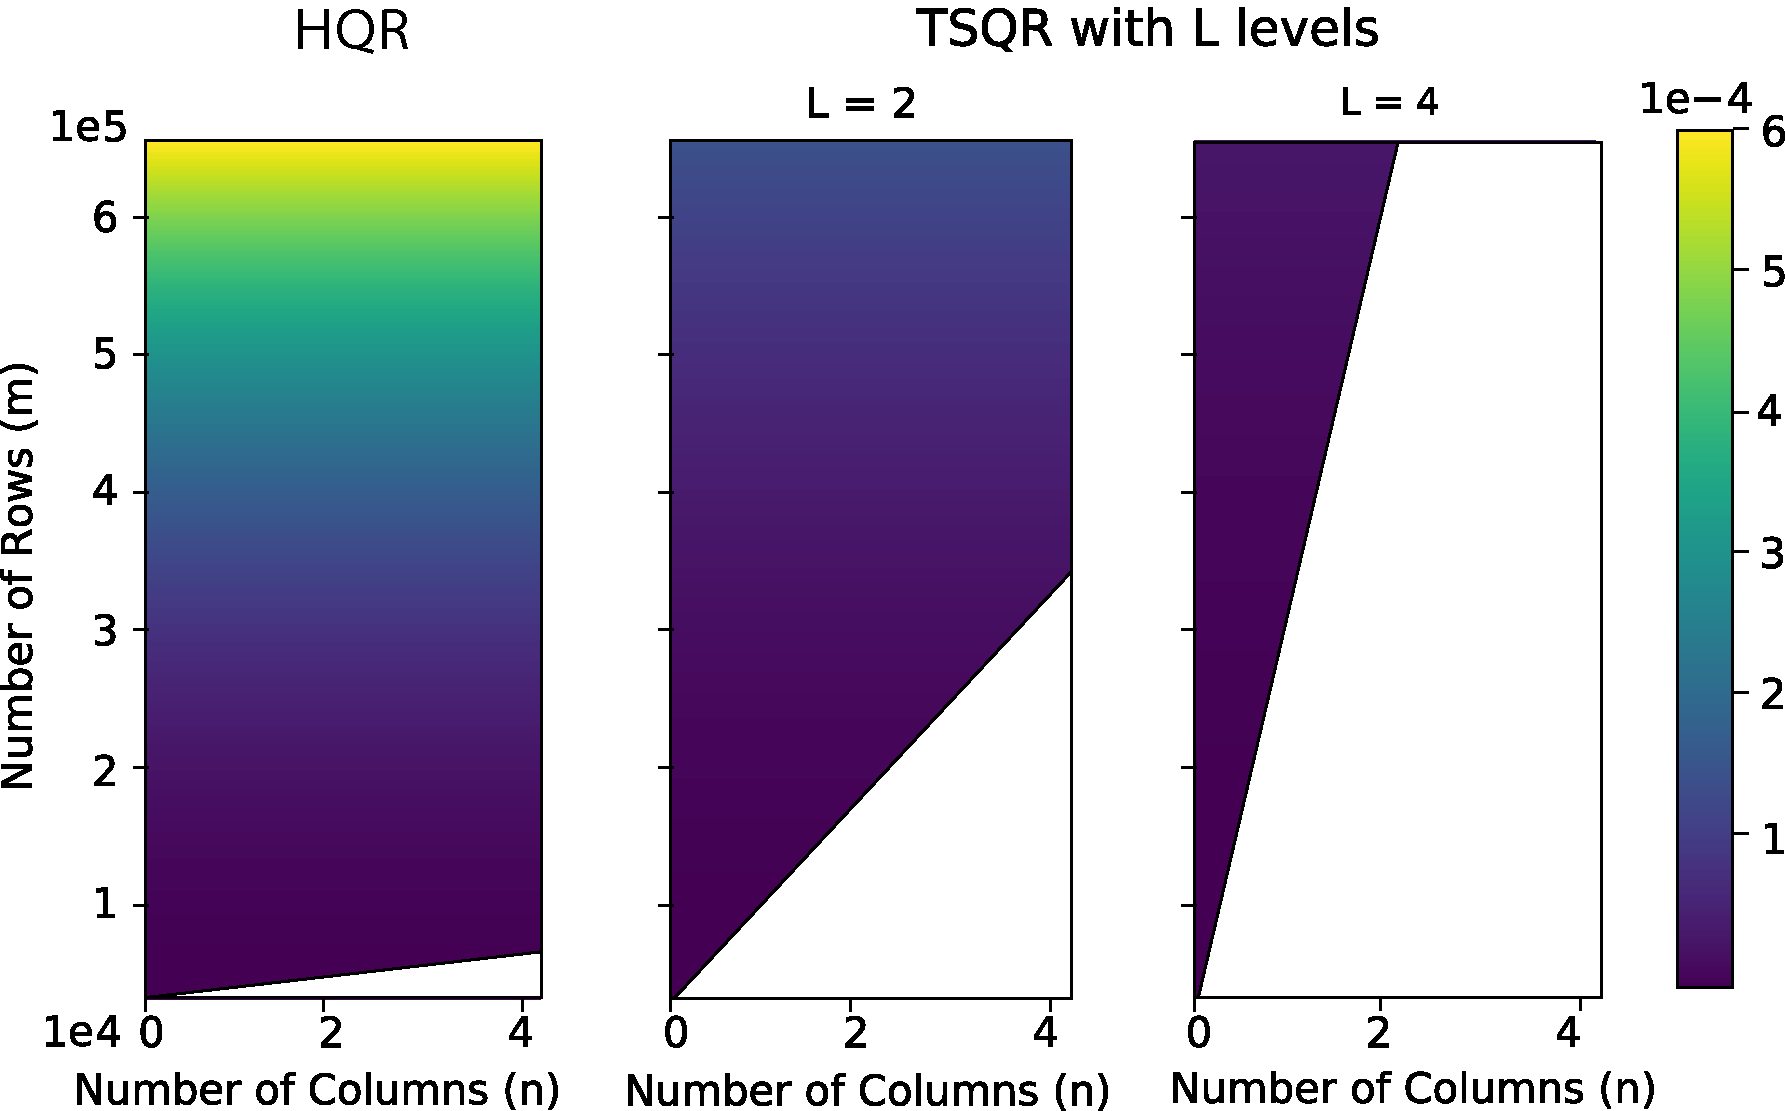
\includegraphics[width=.45\textwidth]{./figures/paramspace.png}
	\caption{\label{fig:paramspace} Non-white space indicates allowable matrix sizes for each scheme, and color map represents error bounds for $\|\bb{\Delta Q}\|_F$ for uniform precision error analysis when using double precision arithmetic.}
	\vspace{-10pt}	
\end{wrapfigure}